% fig11_laurent_contrast.tex
% Contrast: forcing in K (rational-trigonometric) vs in F (Laurent polynomial)
\documentclass[tikz,border=5pt]{standalone}
\usepackage{amsmath,amssymb}
\usetikzlibrary{arrows.meta,decorations.pathreplacing,calc,positioning}

\definecolor{accent}{RGB}{0, 100, 170}
\definecolor{highlight}{RGB}{200, 60, 30}
\definecolor{darkgreen}{RGB}{0, 120, 60}
\definecolor{earthblue}{RGB}{40,80,150}
\definecolor{orbitgray}{RGB}{100,100,100}

\begin{document}
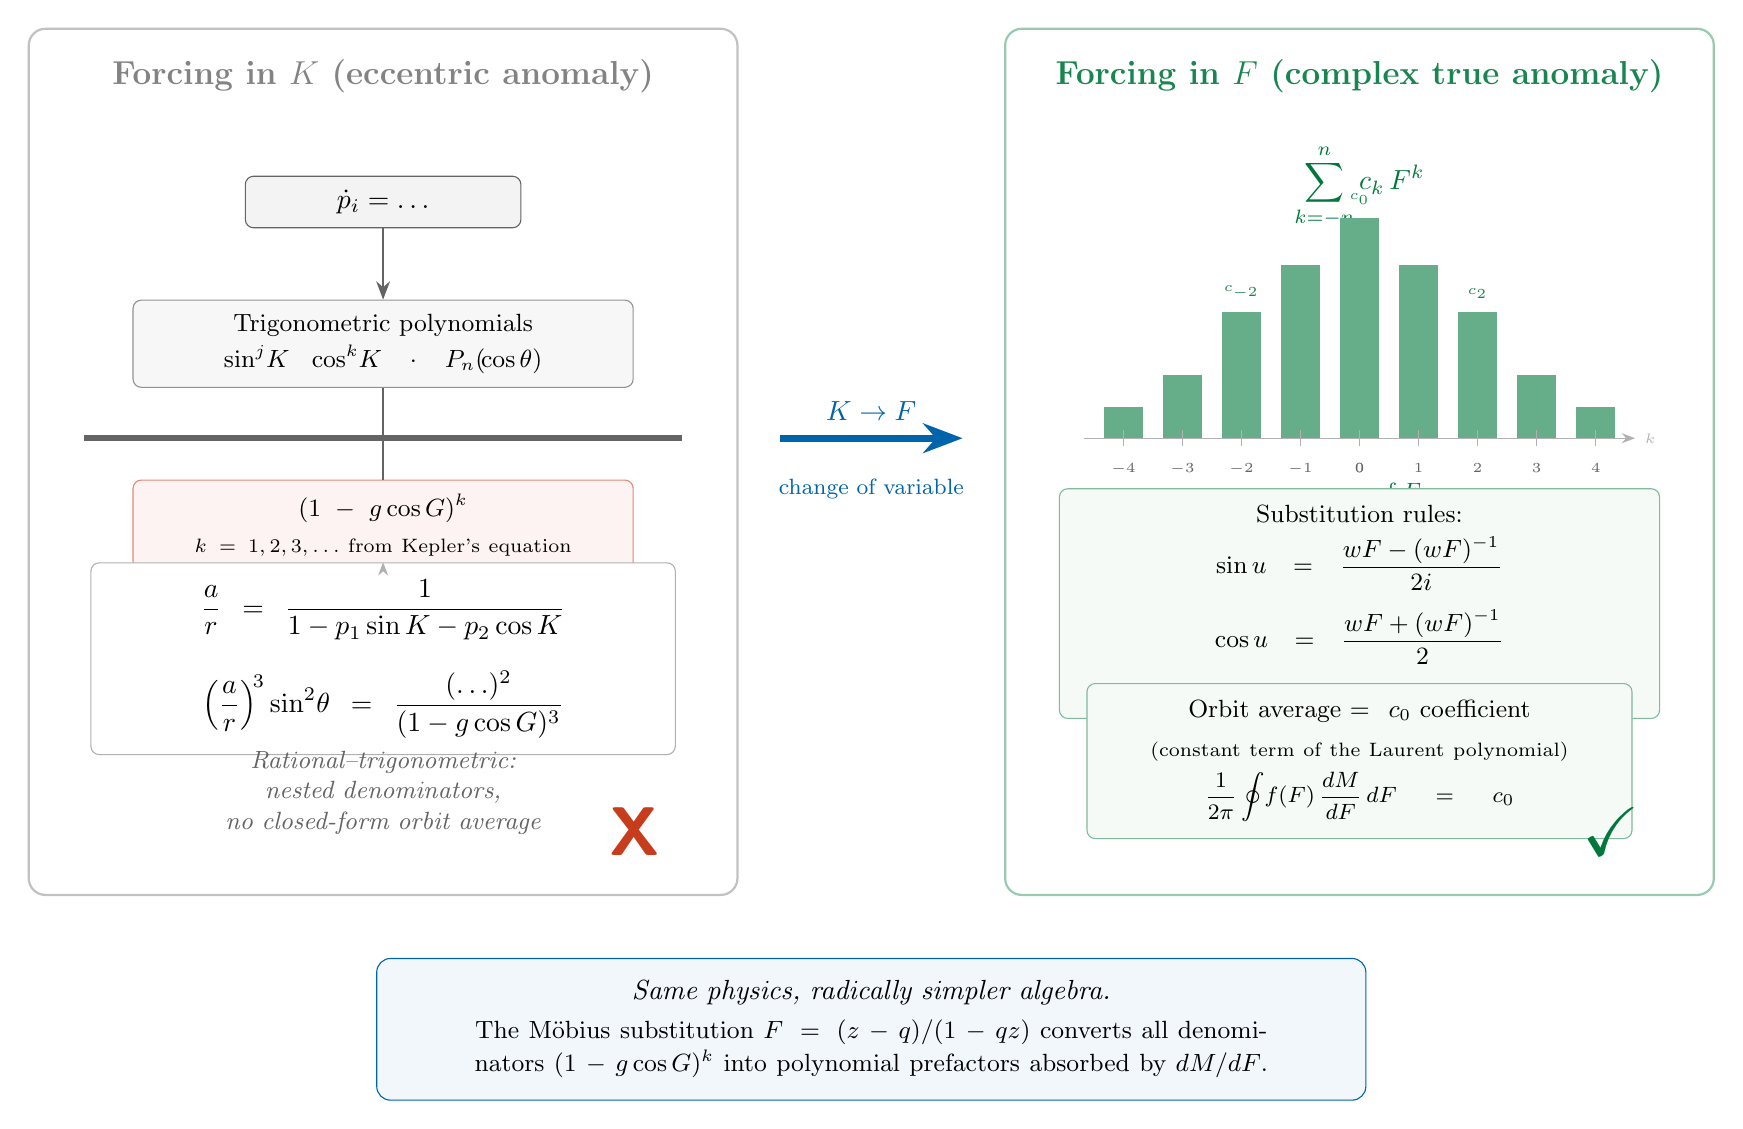
\begin{tikzpicture}[>=Stealth, font=\small]

  % ============================================================
  % LEFT PANEL: Forcing in K (messy rational-trigonometric)
  % ============================================================
  \begin{scope}[shift={(-6.2,0)}]

    % Panel border
    \draw[orbitgray!40, rounded corners=6pt, line width=0.8pt]
      (-4.5,-5.5) rectangle (4.5,5.5);

    % Title
    \node[font=\large\bfseries, orbitgray!80] at (0,4.9)
      {Forcing in $K$ (eccentric anomaly)};

    % --- Expression tree / nested fraction diagram ---
    % Root node: the full RHS
    \node[draw=orbitgray, rounded corners=3pt, fill=orbitgray!8,
          inner sep=5pt, font=\normalsize, minimum width=3.5cm]
      (rhs) at (0,3.3) {$\dot{p}_i = \ldots$};

    % Numerator branch
    \node[draw=orbitgray!70, rounded corners=3pt, fill=orbitgray!5,
          inner sep=5pt, font=\small, text width=6cm, align=center]
      (num) at (0,1.5) {%
      Trigonometric polynomials\\[2pt]
      $\sin^j\!K\;\cos^k\!K\;\cdot\;
       P_n(\!\cos\theta)$};

    % Division line
    \draw[orbitgray, line width=2pt] (-3.8,0.3) -- (3.8,0.3);

    % Denominator branch
    \node[draw=highlight!60, rounded corners=3pt, fill=highlight!6,
          inner sep=5pt, font=\small, text width=6cm, align=center]
      (den) at (0,-0.8) {%
      $(1 - g\cos G)^k$\\[2pt]
      {\scriptsize $k = 1,2,3,\ldots$ from Kepler's equation}};

    % Arrows
    \draw[orbitgray, thick, ->] (rhs) -- (num);
    \draw[orbitgray, thick] (num) -- (0,0.3);
    \draw[orbitgray, thick] (0,0.3) -- (den);

    % Show an explicit example
    \node[draw=orbitgray!50, rounded corners=3pt, fill=white,
          inner sep=6pt, font=\normalsize, text width=7cm, align=center]
      (example) at (0,-2.5) {%
      $\displaystyle\frac{a}{r} = \frac{1}{1 - p_1\sin K - p_2\cos K}$\\[10pt]
      $\displaystyle\left(\frac{a}{r}\right)^{\!3}\sin^2\!\theta
       = \frac{(\ldots)^2}{(1-g\cos G)^3}$
    };

    \draw[orbitgray!50, dashed, ->] (den) -- (example);

    % Label
    \node[font=\small\itshape, orbitgray, text width=6cm, align=center]
      at (0,-4.2) {Rational--trigonometric:\\
      nested denominators, \\
      no closed-form orbit average};

    % Red X mark
    \node[font=\Huge, highlight] at (3.2,-4.7) {\textsf{\textbf{X}}};

  \end{scope}

  % ============================================================
  % RIGHT PANEL: Forcing in F (clean Laurent polynomial)
  % ============================================================
  \begin{scope}[shift={(6.2,0)}]

    % Panel border
    \draw[darkgreen!40, rounded corners=6pt, line width=0.8pt]
      (-4.5,-5.5) rectangle (4.5,5.5);

    % Title
    \node[font=\large\bfseries, darkgreen!90] at (0,4.9)
      {Forcing in $F$ (complex true anomaly)};

    % --- Laurent spectrum bar chart ---
    \node[font=\normalsize, darkgreen] at (0,3.5)
      {$\displaystyle\sum_{k=-n}^{n} c_k\, F^k$};

    % Horizontal axis
    \draw[orbitgray!50, thin, ->] (-3.5,0.3) -- (3.5,0.3)
      node[right, font=\tiny] {$k$};
    % Baseline label
    \node[orbitgray, font=\tiny, below] at (0,0.1) {$0$};

    % Tick marks and bars
    % Coefficients (schematic magnitudes)
    % k:   -4   -3   -2   -1    0    1    2    3    4
    \foreach \k/\h/\lab in {%
      -4/0.4/{-4}, -3/0.8/{-3}, -2/1.6/{-2}, -1/2.2/{-1},
       0/2.8/{ 0},  1/2.2/{ 1},  2/1.6/{ 2},  3/0.8/{ 3},  4/0.4/{ 4}} {
      \pgfmathsetmacro{\xpos}{\k*0.75}
      % Bar
      \fill[darkgreen!60] ({\xpos-0.25},0.3) rectangle ({\xpos+0.25},{0.3+\h});
      % Tick
      \draw[orbitgray!50, thin] (\xpos,0.2) -- (\xpos,0.4);
      % Label
      \node[font=\tiny, orbitgray, below] at (\xpos,0.1) {$\lab$};
    }

    % Coefficient labels
    \node[font=\scriptsize, darkgreen!80, above] at (0,3.15) {};
    \foreach \k/\h in {-2/1.6, 0/2.8, 2/1.6} {
      \pgfmathsetmacro{\xpos}{\k*0.75}
      \node[font=\tiny, darkgreen!90, above] at (\xpos,{0.3+\h+0.05}) {$c_{\k}$};
    }

    % Axis label
    \node[font=\footnotesize, darkgreen] at (0,-0.4) {powers of $F$};

    % Conversion formulas
    \node[draw=darkgreen!50, rounded corners=3pt, fill=darkgreen!4,
          inner sep=6pt, font=\small, text width=7.2cm, align=center]
      (conv) at (0,-1.8) {%
      Substitution rules:\\[4pt]
      $\displaystyle\sin u = \frac{wF - (wF)^{-1}}{2i}$\\[6pt]
      $\displaystyle\cos u = \frac{wF + (wF)^{-1}}{2}$\\[6pt]
      {\scriptsize where $w = e^{i\omega}$ and $F = e^{if}$}
    };

    % Key property
    \node[draw=darkgreen!50, rounded corners=3pt, fill=darkgreen!4,
          inner sep=6pt, font=\small, text width=6.5cm, align=center]
      at (0,-3.8) {%
      Orbit average $= c_0$ coefficient\\[3pt]
      {\scriptsize (constant term of the Laurent polynomial)}\\[3pt]
      {\footnotesize $\displaystyle\frac{1}{2\pi}\oint \! f(F)\,\frac{dM}{dF}\,dF
         \;=\; c_0$}
    };

    % Green checkmark
    \node[font=\Huge, darkgreen] at (3.2,-4.7) {$\checkmark$};

  \end{scope}

  % ============================================================
  % CONNECTING ARROW between panels
  % ============================================================
  \draw[accent, line width=2.5pt, ->, shorten >=4pt, shorten <=4pt]
    (-1.3,0.3) -- node[above, font=\normalsize\bfseries, accent, yshift=2pt]
    {$K \to F$} (1.3,0.3);

  \node[accent, font=\footnotesize, below] at (0,-0.1)
    {change of variable};

  % ============================================================
  % BOTTOM ANNOTATION
  % ============================================================
  \node[draw=accent, rounded corners=5pt, fill=accent!5,
        inner sep=8pt, font=\normalsize\itshape,
        text width=12cm, align=center, anchor=north]
    at (0,-6.3) {%
    Same physics, radically simpler algebra.\\[2pt]
    {\small\upshape The M\"obius substitution $F = (z-q)/(1-qz)$
     converts all denominators $(1-g\cos G)^k$ into polynomial
     prefactors absorbed by $dM/dF$.}
  };

\end{tikzpicture}
\end{document}
